\newpage \chapter{\textbf{Queueing Network Model}}

Then we have identified the physical nodes of our system going to introduce how the Execution Graphs are connected to them:
\bigskip
\bigskip
\bigskip
\bigskip
\begin{center}
\makebox[\textwidth]{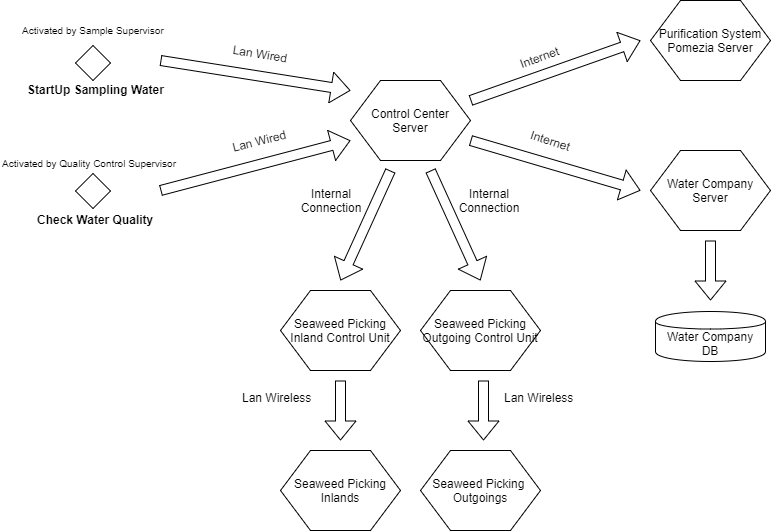
\includegraphics[width=\textwidth]				{PhysicalNodes.png}}
\end{center}
\bigskip
\captionof{figure}{Physical Nodes}

\newpage
This is the Queueing Network so obtained:
\bigskip
\begin{center}
\makebox[\textwidth]{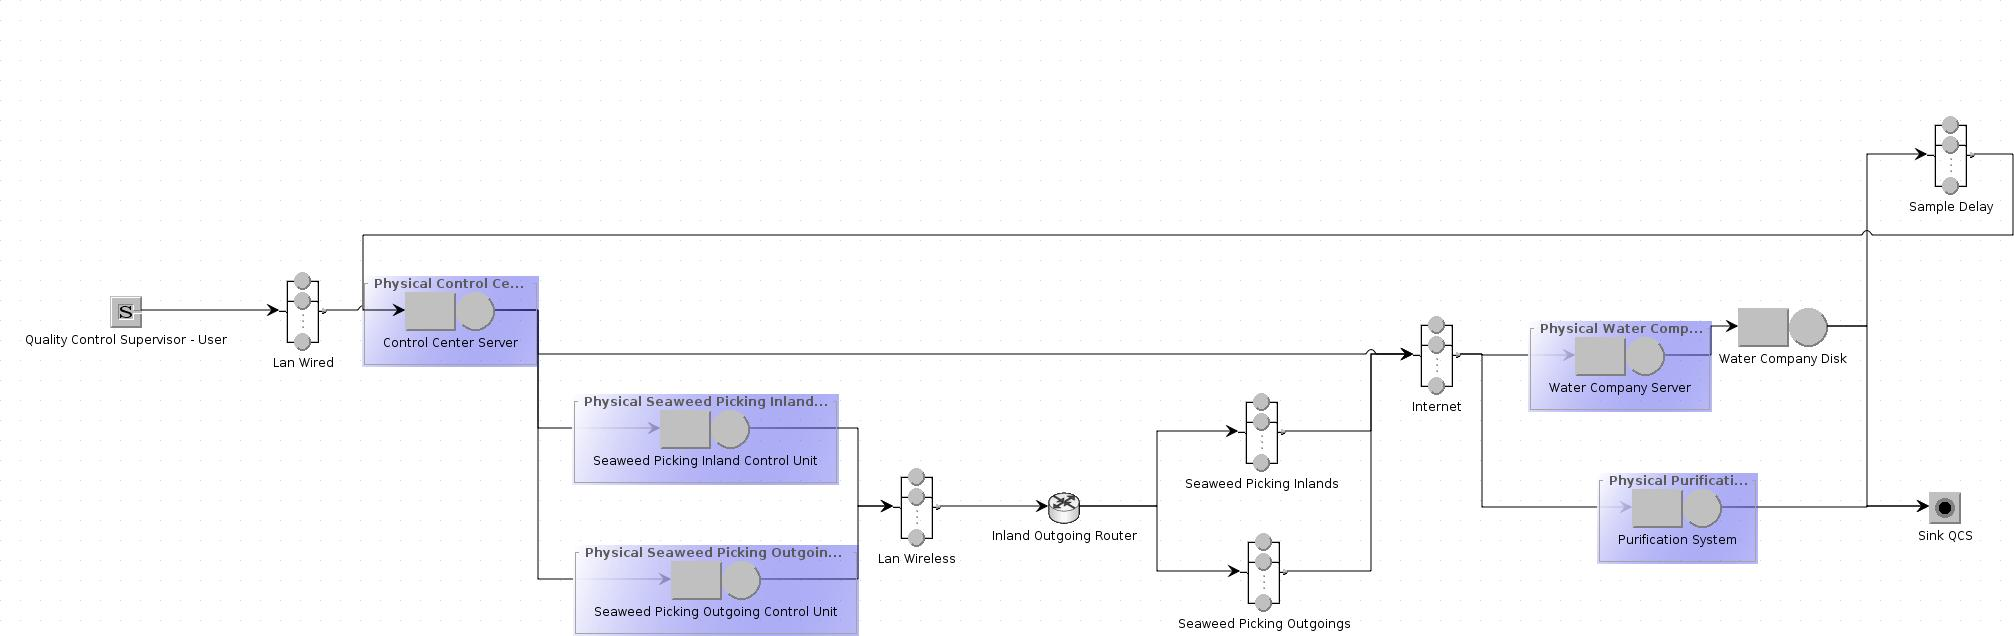
\includegraphics[width=\textwidth]				{QueueingNetwork.jpg}}
\end{center}
\bigskip
\captionof{figure}{Queueing Network}

\bigskip
After several tests, we agreed to reduce the sampling time to 500 seconds to refine the performance analysis. On JMT for the same reason we have only one SeaweedPicking Control Unit and no two for In / Out.\\
We have also decided to eliminate the finite capacity regions as useless for the purposes of our project. So our final Queueing Network has become this:
 
\bigskip
\bigskip
\bigskip
\begin{center}
\makebox[\textwidth]{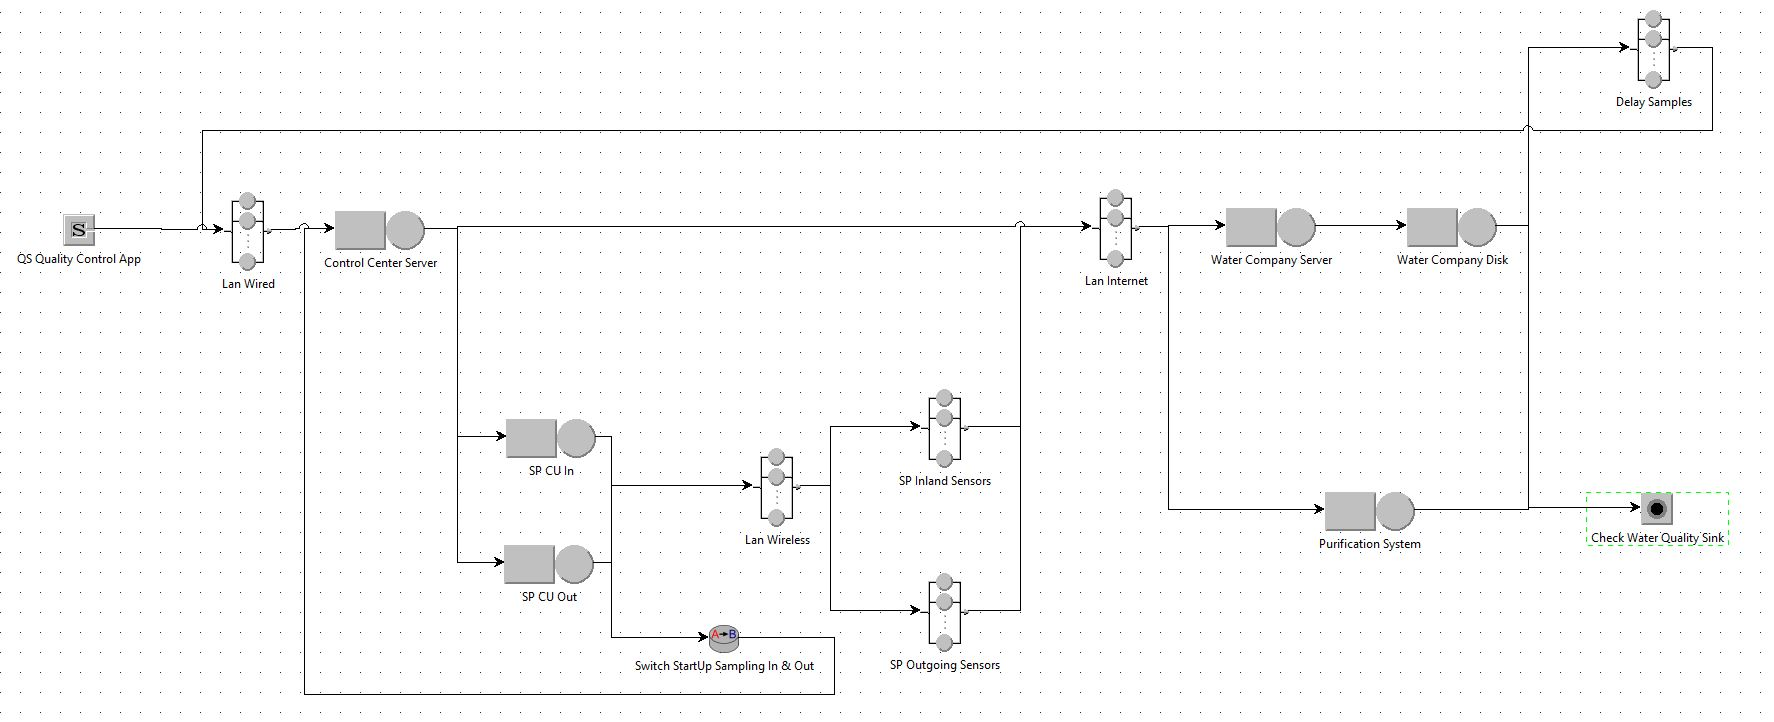
\includegraphics[width=\textwidth]				{QueuingNetworkFinal.jpg}}
\end{center}
\bigskip
\captionof{figure}{Final Queueing Network}